%% It is just an empty TeX file.
%% Write your code here.
\chapter{Dependability} \label{ch:dep}

%************************************************************************************************************************%
\section{Taxonomy} \label{sec:tax}

What makes a system dependable and what does dependability actually mean? \\

\begin{figure}[H]
\centering
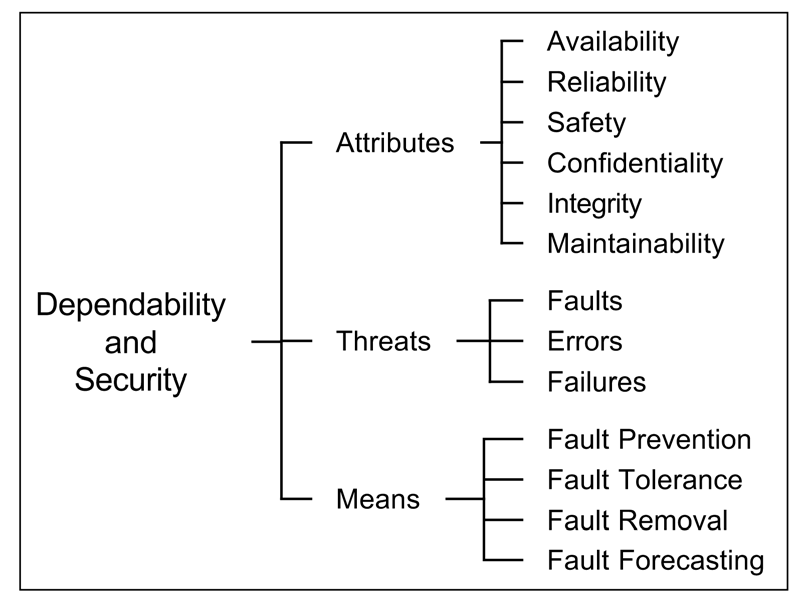
\includegraphics[width=0.65\textwidth]{figures/DepTax.PNG}
\caption{Dependability Taxonomy~\cite{art:Avizienis}}
\label{fig:deptax}
\end{figure}

The dependable system is a system, which has the ability to deliver it's service with acceptable number and severity of system failures~\cite{art:Avizienis}. Dependability ensures then the quality of the system's service~\cite{art:Laprie}. Above all the dependability is an integrating term that encapsulates following \textbf{attributes}:
\begin{itemize}
\item \textbf{availability} - readiness for the delivery of correct service, can be used as a  measure, being a time function $A(t)$ showing the probability that the system functions correctly at the particular time $t$. 
\item \textbf{reliability} - permanence in the delivery of correct service, can also be used as a measure, being the time function $R(t)$ showing the probability that the system has functioned correctly in the time interval $[t_0,t]$ under assumption that it has functioned correctly at the time $t_0$.
\item \textbf{safety} - absence of catastrophic system failures and ability to transit and reside in the fail-safe state, again a measure being a time function $S(t)$ showing probability that a system that worked correctly at time $t_0$ works correctly in the interval $[t_0,t]$ or remains in the fail-safe state,
\item \textbf{maintainability} - possibility of the system alteration and repairs (by authorized subjects) given as a time function $M(t)$ showing the probability that a faulty system will be repaired within time $t$~\cite{art:Laprie, art:Avizienis, art:Avizienis2}.
\end{itemize}
The mentioned above definitions are based on two important terms: system failure and correct service, being in fact antonyms. The absence of one means the presence of the other. A system failure is therefore one of the impairments that threaten the dependability. There are three \textbf{threats}, that form a hierarchical structure:
\begin{itemize}
    \item \textbf{failure} - a state when system delivers service that deviates from the functional specification or the specification describes systems function not adequately; also a transition from a correct state to the described state. Failure happens as a consequence of an error.
    \item \textbf{error} - part of the system state, which may lead to the system failure, but doesn't have to. An error may be latent (after the fault occurrence) or get activated and become effective,
    \item \textbf{fault} - a primary term, an undesired circumstance affecting the system, being a cause of an error~\cite{art:Avizienis, art:Avizienis2}. 
\end{itemize}
An example seems appropriate to illustrate the differences and relationship between dependability threats. 

Let's consider a short-circuit within an integrated circuit and call it a fault. The result of the short, being one of the connections stuck at a boolean value - an error. The error remains latent until it doesn't get activated. In this scenario the activation would be an attempt of a logical switch of this connection to the opposite value, causing a failure of the connection - an obvious deviation from the specified behavior (reproduction of the input signal to the output of the connection). But a failure of one connection doesn't [have to] mean a failure of the whole integrated circuit. The hierarchical structure of dependability threats and a general hierarchical structure of systems results in the cause and effect relationship called error propagation. It is illustrated in the \autoref{fig:propagation}. An error gets internally propagated until it reaches the interface of another systems component. The failure of one component creates an error in the interfaced component. If this error leads to incorrect service of the entire system, then it means the system failure occurred~\cite{art:Avizienis, art:Avizienis2}. \\

\begin{figure}[H]
\centering
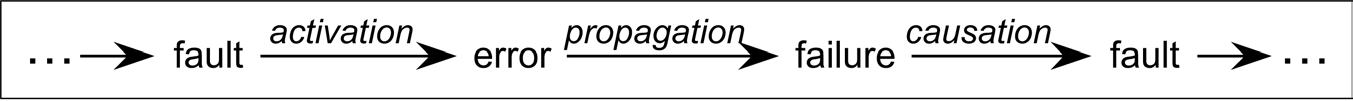
\includegraphics[width=0.65\textwidth]{figures/propagation.png}
\caption{The chain of dependability~\cite{art:Avizienis}}
\label{fig:propagation}
\end{figure}

Knowing what the dependability is and what are the threats it is important to know what available \textbf{means} do developer have to create a dependable system. There are four solutions:
\begin{itemize}
    \item \textbf{Fault Prevention} aims mostly at the development phase of a system and relays on design rules, modularization and strongly-typed languages. It also records the detected faults and eliminates them through development process modification.
    \item \textbf{Fault Tolerance} stands for methods which imply the presence of faults and their inevitability. Hence the need for error detection and processing. The fault tolerance is elaborated in the~\autoref{sec:tolerance}.
    \item \textbf{Fault Removal} in the development phase has three stages: verification, diagnosis and correction. If the verification shows faults in the system, the two other steps need to by applied. The verification needs to be repeated afterwards. In the use phase the faults are removed through maintenance, which requires an external agent (a repairman, some test equipment or software).
    \item \textbf{Fault Forecasting} bases on evaluation process of the system behavior, especially the fault occurrence and activation. The evaluation can be either qualitative - classify and rank events that are dangerous to the system; or quantitative - count and give probabilistic measure of the extent in which the attributes of dependability are satisfied~\cite{art:Avizienis, art:Avizienis2}. 
\end{itemize}
While the fault prevention and the fault forecasting are more useful in analysis of the system dependability and aim to minimize the amount and severity of faults in the system, thus helping by the fault avoidance; the fault tolerance and fault removal both assume that the faults happen and provide methods to reduce their impact on the system, creating a group of fault acceptance methods, thus helping by handling with systems that are subject to faults. \autoref{fig:depgroup} represents the grouping of dependability means.

\begin{figure}[H]
\centering
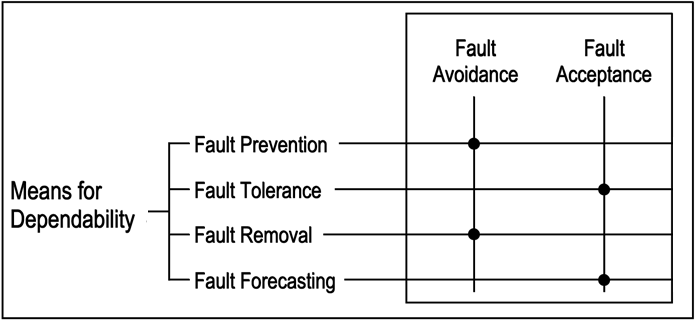
\includegraphics[width=0.65\textwidth]{figures/depgroup.png}
\caption{Grouping of the means for dependability~\cite{art:Avizienis}}
\label{fig:depgroup}
\end{figure}

%************************************************************************************************************************%
\section{Fault Pathology}
There are eight categories that help to understand what kinds of faults there are and how they may influence the system. They are called the elementary fault classes. Each fault falls into more classes. They may be understood as properties of a fault. The possible combinations are marked with a dot in the~\autoref{fig:fault}. The developer has to decide witch classes should be included in the dependability specification.

\begin{figure}[H]
\centering
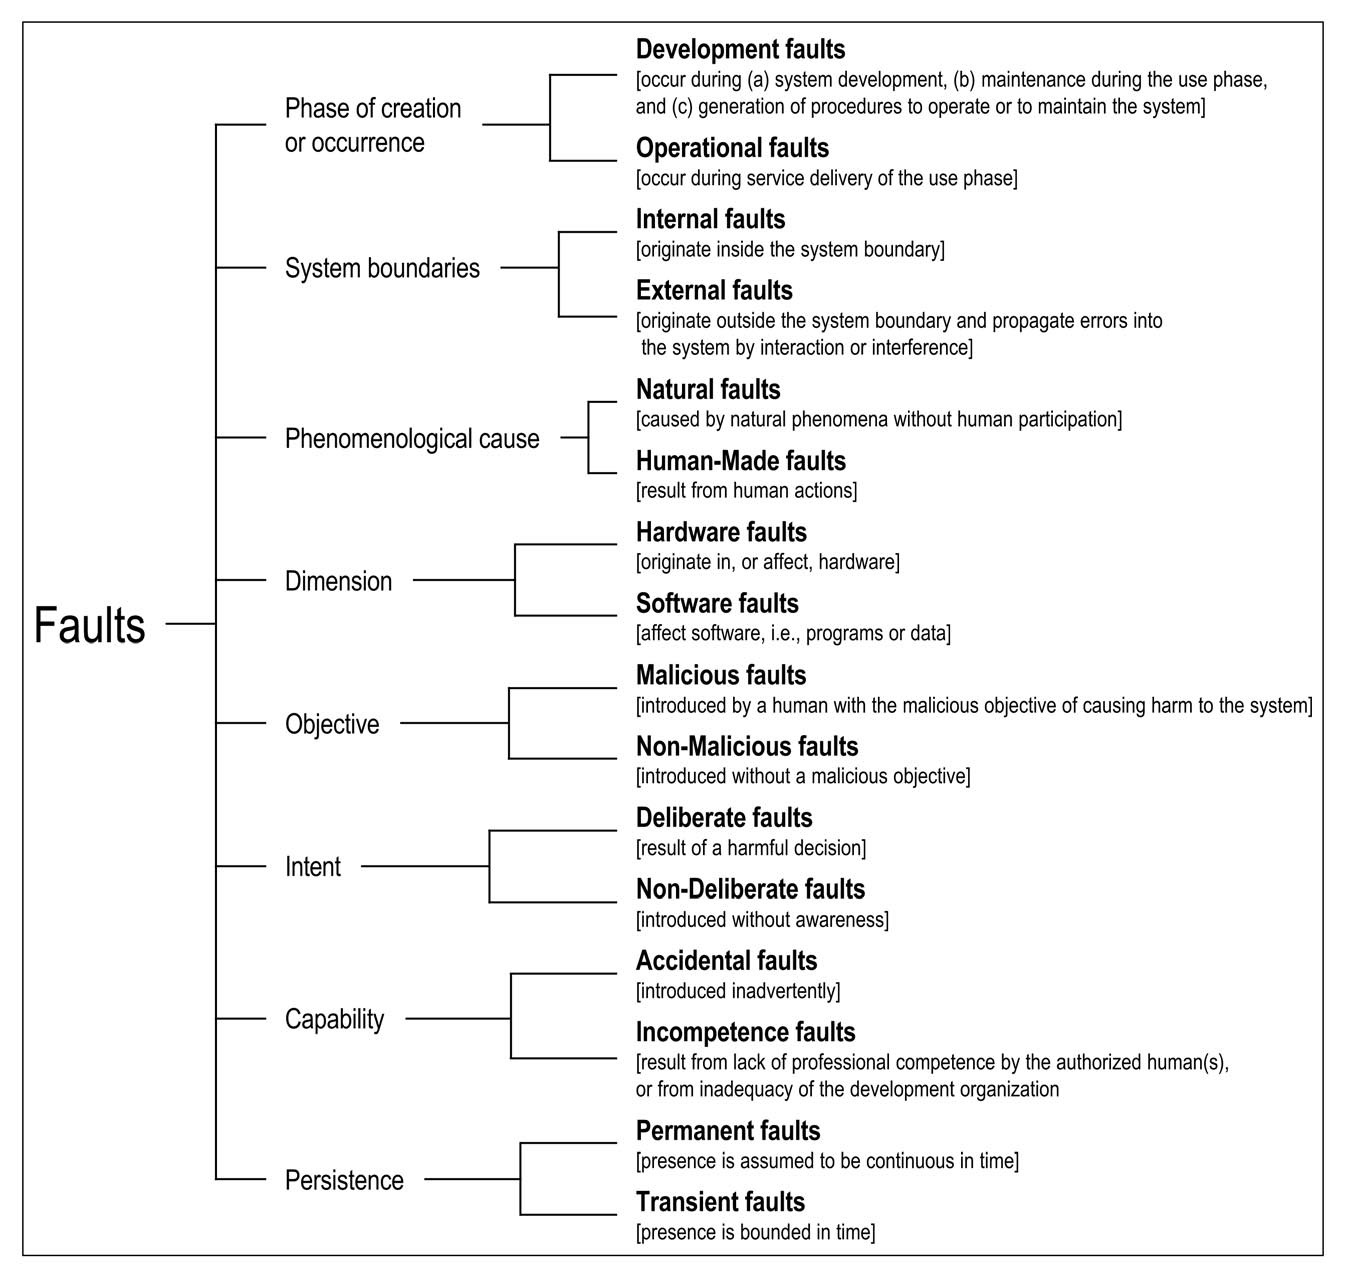
\includegraphics[width=0.65\textwidth]{figures/fault.png}
\caption{The elementary fault classes~\cite{art:Avizienis}}
\label{fig:fault}
\end{figure}

The classes divide into three main groups: the development faults, the physical faults and the interaction faults. The development faults occur during the development phase of the system. The last group describes faults that happen during the use phase and come from the use environment of the system, hence they are operational faults. Physical faults are all faults that happen in hardware, they happen during the development and use phase invariably.
Very important perspective splits faults up into two, or actually three groups, based on the duration of the fault and its persistence:
\begin{itemize}
    \item The \textbf{transient faults} occur once and don't persist afterwards. The error caused by such a fault is called a soft error.
    \item The \textbf{permanent faults}, often called hard faults, occur at some point in time and last until the faulty component gets repaired. Faults occurrence may happen already in the development phase and results in erroneous data being produced by affected component during its use. 
    \item The \textbf{intermittent faults} occur repeatedly but not continuously in the same spot in the design. The errors caused by such faults tend to also be intermittent~\cite{book:Sorin}.
\end{itemize}
The knowledge about the faults persistence is therefore important, that it changes the strategy of fault tolerance. The permanent faults, to be removed, require some sort of repair procedure, while the transient faults require much less complicated treatment, like repetition of the operation.

Let's focus on faults that occur in hardware and are caused by natural phenomena. Those faults are marked with a box in the~\autoref{fig:fault}. There are three stages within this group:
\begin{itemize}
    \item Production defects - are all development faults which are permanent. These can be imperfections and variations in one of the production stages or dust particles causing shorts. They lead to functional and parametric errors and should be caught before the use phase. One of the possibilities is the burn-in test which consists in stressing the circuit with high temperature and voltage, leading to its premature aging. The early life failures are caught and affected circuit doesn't get to it's use phase.
    \item Physical Interference - are all external faults, both permanent, transient and intermittent caused by radioactive radiation and electromagnetic interference. These faults are randomly distributed throughout the whole life of a the system.
    \item Physical Deterioration - are the faults resulting from aging. They can be permanent, transient and intermittent. Electromigration (EM) and Stress Migration (SM) are just two of many possible aging effects by which an integrated circuit may be affected. The probability of such faults rises together with the systems age~\cite{art:Avizienis, art:Avizienis2}.
\end{itemize}
The~\autoref{fig:badewanne} shows the Fault rate/time relation. The first part of the diagram shows Early-Life-Failures, which result from the Production Defects. They should be captured during early life tests of the design. Next stage shows all faults happening due to Physical Interference. They are constantly threatening the system keeping the fault rate at the stable level. It may happen that systems environment is less or more "fault likely" but it would just shift the fault rate along the $y$ axis and not change its monotonicity. The last part shows a rising number of faults due to aging and deterioration processes happening to every hardware (and, according to some definitions also to software).

\begin{figure}[H]
\centering
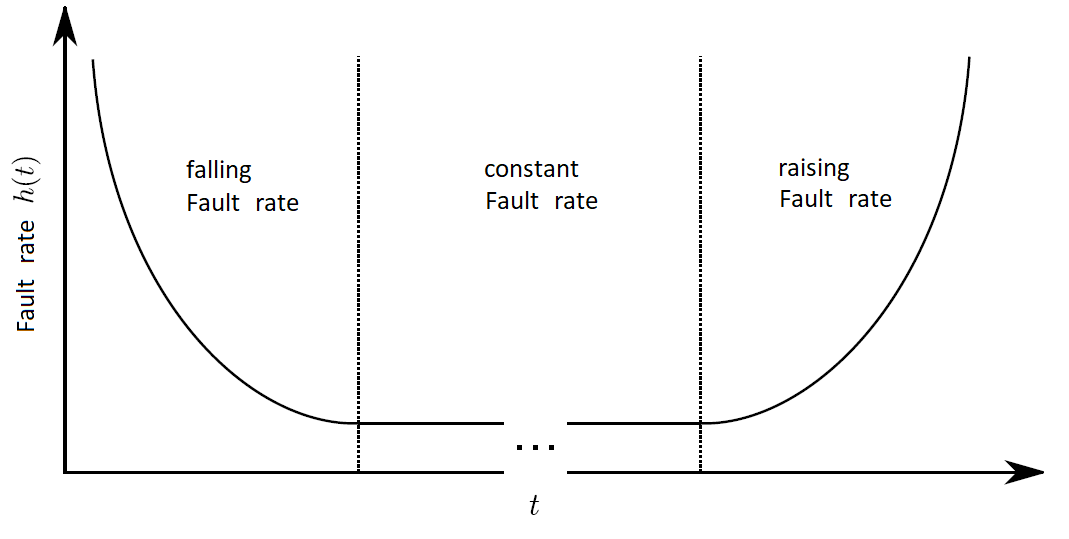
\includegraphics[width=0.65\textwidth]{figures/badewanne.png}
\caption{Fault rate throughout systems life cycle~\cite{art:Avizienis}}
\label{fig:badewanne}
\end{figure}


%************************************************************************************************************************%
\section{Fault Tolerance}
The fault tolerance is one of the dependability means. The developer cannot only rely on fault avoidance methods because of the time needed for manual repair and frequency of those repairs. Sometimes the system is also inaccessible for maintenance. Additionally the more complex is the hardware, the more liable it is to natural faults. Thus while designing the hardware which is either very complex or doesn't allow long times to repair then the incorporation of fault tolerance is a must.\\
Fault tolerant systems can react differently in the presence of faults. Some provide the full performance, some offer just a reduced functional capability~\cite{art:Randell}. There are therefore different schemes of fault tolerance and they depend on the faults that are supposed to be tolerated. There are however two main parts that have to always exist: error detection and system recovery.\\
The error detection can either be concurrent to main functionality or happen during scheduled pauses, when normal functionality is suspended. After the error is detected the recovery routine has to deal with two problems. The first one is the error handling which can be performed via:
\begin{itemize}
    \item backward error recovery - executed on demand. The system is brought back to a saved state that is known to be error-free. This state has to be saved prior to error occurrence, thus its name is checkpoint.
    \item forward error recovery - also executed on demand. Finding a new state, which has not yet bee occupied by the system, which is error-free.
    \item error compensation - can be used either systematically (also in absence of faults) or on demand. The erroneous state contains enough redundancy to provide correct service despite the fault. The systematic usage is called the fault masking.
\end{itemize} 
The other problem is to remove the cause of an error, therefore the fault handling may be necessary. It consists of:
\begin{itemize}
    \item Diagnosis - identifies and stores the cause of an error and its location together with the time when the error happened.
    \item Isolation - excludes the faulty component from normal function either logically or physically 
    \item Reconfiguration - provides a spare component to take place of the faulty one or reassigns the tasks among non faulty components
    \item Reinitialization - logs the changes made in configuration and updates the records or system tables 
\end{itemize}
The coverage of fault tolerance is a measure of its successful detection of erroneous states associated with faults and its ability to repair or replace such states. Every method covers different faults and errors, therefore only a combination of them can lead to a maximum fault coverage.
Fault tolerance requires protective redundancy, being additional components and algorithms allowing the error detection and preventing errors from leading to failures. Unfortunately the fault tolerance is a recursive procedure, witch means that every redundancy, when implemented, becomes part of the system, and therefore can be affected by all previously described faults.
There are four main arts of redundancy: time redundancy, hardware redundancy, software redundancy and information redundancy. The software redundancy will not be discussed.
%************************************************************************************************************************%
\subsection{Hardware Redundancy} \label{ssec:HWred}
The main overhead lies in hardware. The components are either passive or active. 

The passive redundancy aims for immediate masking of a failure. As long as the number of faults doesn't exceed the specified maximum, the system provides correct functionality without showing any kinds of disturbance. It's achieved through a parallel execution of operations on more concurrent components in hope that faults appear independently in each one of them. An example of such art of redundancy is the N-Modular Redundancy system, which has N modules running in parallel and majority voter that propagates the result that occurred in the majority of the modules. A variation of such system would incorporate more voters running in parallel to eliminate the single-point-of-failure, which is the voter in an NMR system. Passive redundancy is an example of error compensation without any sort of fault handling and systematic error detection, which happens inside of the voter. The permanent faults are masked as long as their accumulation with transient faults doesn't exceed the coverage of the system.

The active redundancy is a way to solve the permanent fault problem which occurs in passive redundancy. After error detection, the erroneous component is localized and replaced by a fault-free spare component. The start procedure of such a component can take some time, that could be avoided if the component had worked in parallel to the rest of the system by the time of error occurrence. Such strategy is called a Hot-Standby (in opposite to Cold-Standby) but it leads to component deterioration, without it being actually used for the main functionality. The active redundancy is an example of rollforward approach, since the configuration after repair is a state that has not been used before the error occurrence. The error detection can be either systematical or happen in intervals, depending on the requirements.

There is a possibility to combine both approaches to a hybrid one. Having a systematical error compensation with an active spare modules. Once a permanent fault is detected a reconfiguration takes place, either on-line or during a break.


%************************************************************************************************************************%
\subsection{Time Redundancy}
This type of redundancy has a very powerful advantage, namely it doesn't require so much additional hardware. The time redundancy is mostly implemented in software, that executes operations more times in a row achieving the same result as the hardware redundancy without its cost. With 2 repetitions the errors can be detected and three repetitions allow error correction. The repetitions can be achieved through a checkpoint system. The repetitions may also happen concurrently on different threads leading to use different processor resources for the same task and creating a quasi NMR system. For transmission errors the \textbf{Error Correction Through Retransmission} is possible. It's based on an assumption, that after the detection of an error, there is enough time to retransmit the information. The redundancy results in the additional control bits for error detection (information redundancy) and in the additional time for retransmission.

%************************************************************************************************************************%
\subsection{Information Redundancy}\label{ssec:Infred}
The information flow through a system can be corrupted by many different faults. Other proposed methods try to not let to the information integrity violation. But maybe even if the information got changed, then there is a possibility to detect this change and reconstruct the original information. The information redundancy tries to achieve exactly this goal by adding some special parity bits to detect or even correct the errors. Special codes make it possible to achieve this goal.
\textit{Backward Error Correction}
Backward Error Correction (BEC), more commonly called Automatic Repeat Request (ARQ) allows the detection of errors in the information and requires the retransmission. The codes used in this approach are called Error Detecting Codes (EDC)
\textit{Forward Error Correction} (FEC) enables localization of the error position within the information and as a result, reconstruction of the original information, without the need of retransmission. The only redundancy are the control bits and the encoder (Hardware or Software). The codes used in this approach are called Error Correcting Codes (ECC)~\cite{book:SchonfeldKlimant}.

%************************************************************************************************************************%
\section{Channel Coding} \label{sec:cod}
In the year 1948 Shannon published a landmarking paper "Mathematical Theory of Communication" where he showed that, with a certain information encoding, the errors induced by a noisy channel can be reduced to any suitable level~\cite{art:Shannon}. With this article he started the era of coding theory and a race to create better and better codes with simple decoding algorithms~\cite{book:Lint}. He laid the mathematical foundation of reliable communication, which gets improved until this day.\\
Channel Coding is, generally speaking, a process of adding useful redundancy to the source information in order to recreate it's contents after it arrives at the sink. The recreation can happen either by simple information retransmission or error correction.
\subsection{Error Detection}
To conduct any error correction, the error detection has to take place first. Some systems are armed only with this mechanism. Let's assume that the information leaving the source encoder is a binary sequence that can be divided into blocks of length $k$. Each block is denoted as $u=\{u_1,u_2,...,u_k\}$ and is called a \textit{message}. Since the information is binary, there are $2^k$ different messages possible. The channel encoder transforms each $message$ into a binary \textit{code word} $v=\{v_1,v_2,...,v_n\}$, with length $n$, where $n\geq k$, since the additional information is being added. There are still only $2^k$ valid \textit{code words}, since every \textit{code word} corresponds exactly to one $message$. The set of all valid \textit{code words} is called a code space. It leaves $2^n - 2^k$ \textit{code words} that are not used in transmission. The ratio $R=k/n$ is called the \textit{code rate} and can be understood as the number of the information bits entering the encoder per transmitted symbol. During the transmission, an \textit{error vector} $e=\{e_1,e_2,...,e_n\}$ overlays the \textit{code word} producing a \textit{received sequence} $r=\{r_1,r_2,...,r_n\}$. If the \textit{received sequence} is not a valid \textit{code word}, then the error gets detected. The worst case scenario is when the \textit{error vector} transforms a \textit{code word} into a valid \textit{received sequence} but different then the \textit{message} sent, $r\neq q$. Then the \textit{received sequence} gets accepted and decoded into wrong $message$. To avoid such situations, the \textit{code words} should lay possibly away from each other. The \textit{hamming distance d} (between two \textit{code words}) is the number of positions, in which both words differ. The number of errors $f_d$, that a code can detect, depends on the minimum hamming distance $d_{min}$ in the code space, which has to satisfy following inequality $d_{min} \geq f_d + 1$.
\subsection{Error Correction}
If the \textit{code word} overlaid with \textit{error vector} results in the \textit{received sequence} outside of the code space, then the error gets detected. The~\autoref{fig:hamming_dist} shows the hamming distance cube for a 3 bit binary word. Each vertex symbolizes a possible \textit{received sequence}, where only words $\{000\}$ and $\{111\}$ are valid \textit{code words}. The distance between the words is equal to the number of edges between them. The hamming distance between the \textit{code words}, being the minimum hamming distance is $d_{min}=3$.

\begin{figure}[H]
\centering
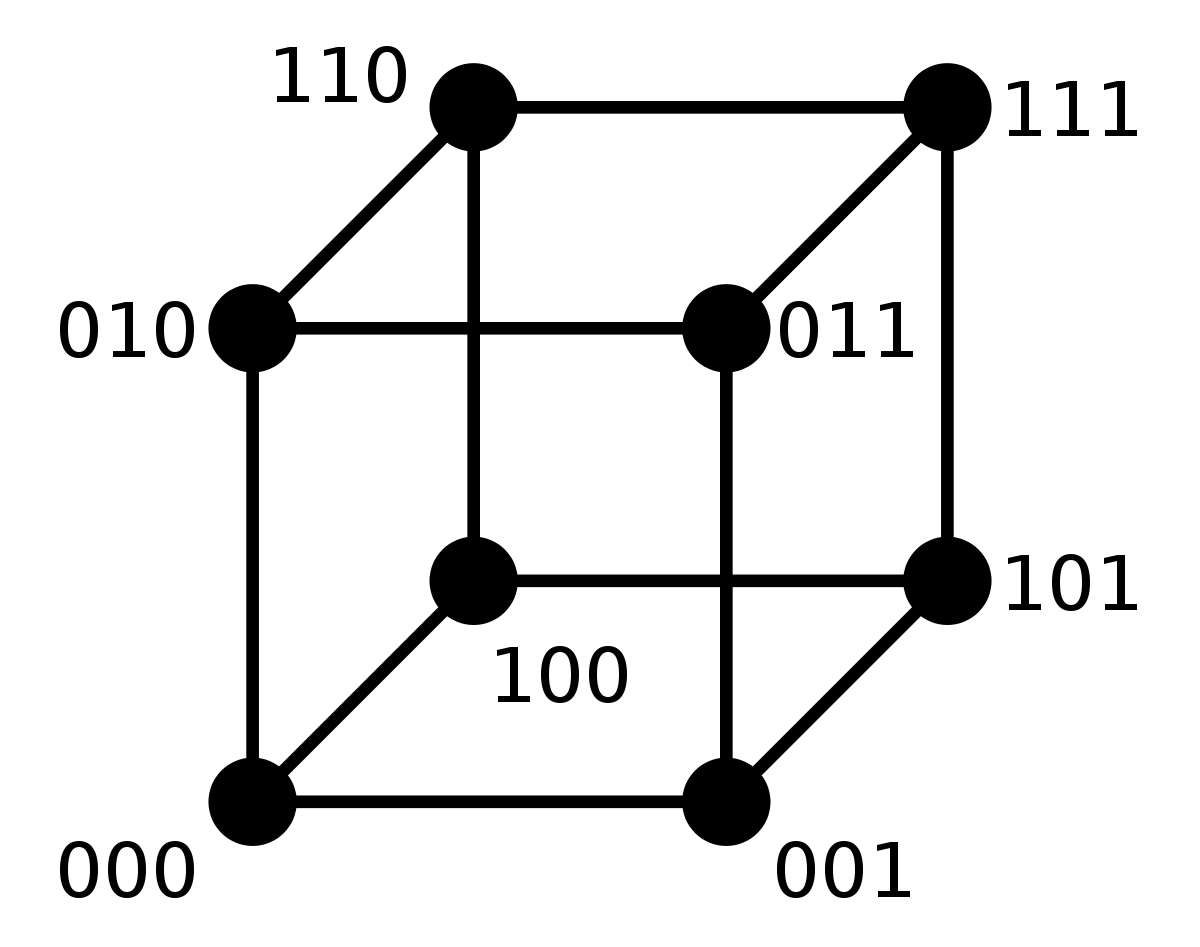
\includegraphics[width=0.3\textwidth]{figures/Hamming_distance.png}
\caption{Hamming distance cube for 3-bit binary numbers~\cite{web:hamming_dist}}
\label{fig:hamming_dist}
\end{figure}

Assuming that the number of errors is $f_c = 1$, then upon reception of erroneous data, the distance between the \textit{received sequence} and valid \textit{code word} will also be $d = 1$. The \textit{received sequences} form two disjoint sets $r_{000}=\{001,010,100\}$ and $r_{111}=\{110,101,011\}$. The reception of any word from each set unambiguously refers to only one valid \textit{code word}. To correct $f_c$ errors the code needs to have $d_{min} >= 2f_c+1$. If the $d_{min}$ is even, then there will always be some words in the \textit{received sequence alphabet} that have equal distance to more than one \textit{code word}. A perfect code is an optimal code, where every \textit{received sequence} can be unambiguously subordinated to a valid \textit{code word}. The code has to satisfy the following equality $k=ld\sum_{i=0}^{f_c} {n \choose i}$ to be called a perfect code. Perfect codes use their redundancy fully, guaranteeing maximal protection by minimal overhead.


